\documentclass[11pt]{article}
\usepackage{amsmath,array}
\usepackage{amsfonts}
\usepackage{amssymb}
\usepackage{amsthm}
\usepackage{breakcites}
\usepackage{graphicx,subcaption}
\usepackage{todonotes} %[disable]
\usepackage{cleveref}
\usepackage{tikz}
\usepackage{placeins} %FloatBarrier
\usepackage{booktabs}
\usepackage{natbib}
\usetikzlibrary{arrows,shapes,calc}
\tikzset{line/.style = {draw, -latex', ultra thick}}
\newcommand{\abs}[1]{\left|{#1}\right|}
\newcommand{\pde}[2]{{\frac{\partial {#1}}{\partial {#2}}}}
\newcommand{\pdde}[2]{\frac{\partial^2 {#1}}{\partial {#2}^2}}
\newcommand{\de}[2]{\frac{\mathrm{d} #1}{\mathrm{d} #2}}
\newcommand{\dde}[2]{\frac{\mathrm{d}^2 {#1}}{\mathrm{d} {#2}^2}}
\newcommand{\intdef}[4]{\int\limits_{#1}^{#2} #3\, \mathrm{d}{#4}}
\newcommand{\mean}[1]{\left<{#1}\right>}
\crefname{appendix}{Appendix}{appendices}
\crefname{section}{Section}{sections}
\crefname{table}{Table}{tables}
\Crefname{table}{Table}{Tables}
\crefname{equation}{Eq.}{eqs.}
\Crefname{equation}{Equation}{Equations}
\crefname{figure}{Fig.}{figs.}
\Crefname{figure}{Figure}{Figures}
\crefname{subfigure}{Fig.}{figs.}
\Crefname{subfigure}{Figure}{figures}
\captionsetup[subfigure]{labelformat=simple}
\renewcommand{\thesubfigure}{(\alph{subfigure})}
\renewcommand{\vec}[1]{\boldsymbol{#1}}
%opening
\title{Inferring causal connectivity from pairwise recordings and optogenetics}
%\title{The need to combine optogenetics with neural recordings to estimate causal connectivity}
\author{Mikkel Elle Lepper\o{}d, Konrad Paul Kording}

\begin{document}

 \maketitle

\begin{abstract}
\noindent Neuroscientists often want to identify how neurons causally interact. Perturbations with optogenetics are a popular way of quantifying such interactions. However, even focused light will typically stimulate multiple cells, which produces a confound - we cannot know which of the stimulated neurons affected the activity of a given target neuron. Here we show how this confound produces large biases in estimates of connectivity, and how we can reduce these biases by a data analysis strategy that exploits the absolute refractory period of neurons. We use the instrumental variable (IV) framework from economics which estimates causal strengths by exploiting a variable that affects only one of the variables, here the presynaptic neuron. The interaction between optogenetic stimulation and the absolute refractory period produces a weak almost random signal (IV) that we exploit to solve the causal inference problem. In a simple simulation of integrate and fire neurons, we find that instrumental variable techniques estimate connectivity better than naive techniques (99.8\% vs 86\% correct). Our instrumental variable approach is robust and easy to implement in the context of current experimental paradigms.
\end{abstract} 

\section{Introduction}
% neuroscience experiments are observational which implicates a certain set of statistical tools
% spike timing cannot give a causal estimate of connectivity, thus we need to perturbe the system
%a quest for causality and optogenetics is a main tool
% We want mechanism. Seriously. Neuroscience is to a large part experimentally driven.
%set up the drive to causality
We want to understand the mechanisms or causal chains that give rise to activity in the brain, to perception, action, and cognition. For such an understanding it is not sufficient to know the correlations between variables or even be able to predict them. After all, there can be many ways how the same activities come about by distinct causal chains \citep{drton2011global, peters2017elements}. Identifiability of causal networks is complicated when it comes to brain data. Complex systems such as the brain are hard to understand because of the numerous ways the contributing elements may interact internally \citep{Jonas2017}. Thus, brain data which is almost always observational, will almost never satisfy the criteria needed for identifiability \citep{pearl2009causality}. While observing correlations within the system is usually relatively easy, transitioning from observed correlations to a causal or mechanistic understanding is hard or, more commonly, impossible.  Getting at such an understanding in the human brain is nearly impossible as it contains approximately 86 billion neurons \citep{azevedo2009equal}, each of which influences many other neurons. Only under certain assumptions about nonlinearity or noise sources does a fully observed system become identifiable \citep{daniusis2012inferring,shimizu2006linear}. Even if we could record all neurons at the same time, estimating causality and producing a mechanistic understanding would be extremely challenging.

% we use observational studies. But causality is typically wrong. 
Moreover, we generally only record from a small subset of all neurons. The data we obtain from typical recordings, e.g. from electrophysiology  or calcium imaging, is very low dimensional relative to the dimensionality of the brain. Moreover, it is observational, which means that it does not result from randomized perturbations. In such cases, we can never know to which level the observed activity was caused by other observed activity, or by the activity of the unobserved neurons. Such unobserved activity is then called confounders. If mechanisms are estimated from observational data in the presence of confounders, we will generally make large errors and draw incorrect conclusions \citep{angrist2008mostly}. Unobserved neural activity confounds estimates of causal interactions and makes it difficult to estimate underlying mechanisms.

%set up confounding
Confounding is the big threat to causal validity \citep{UpcomingMehlerPaper} irrespective of the use of simple regression techniques or advanced functional connectivity techniques \citep{stevenson2008inferring, honey2009predicting, aitchison2017or, pfau2013robust}.  A much used method for estimating the output of single neurons is to perform multiple regression analyses \citep{pillow2008spatio}, modeling each neuron with a generalized linear model (GLM).  Multiple regression may be perceived as a solution to confounding problems as they support the concept of ``explaining away" \citep{stevenson2008inferring}. However, in current work we will exclude approaches that look at multiple neurons at the same time. This is because, ``explaining away" can only be a good strategy if most neurons are included in the recordings but this is rarely the case for most experimental settings, especially in the mammalian brain. We will therefore focus on neuron pairs where stimulus and the pre- and post-synaptic neurons are known.

To estimate connectivity it is first and foremost important that it stems from cause and effect e.g. B's action potential is causing an increase in C's membrane potential, therefore we use the term causal connectivity.  For a given example we want to estimate causal connectivity between two neurons, $ A $ and $ C $ (\cref{fig:intro}\labelcref{fig:intro:1}). Two neurons, $ A $ and $ B $, are driven by a common input $ D $ and because $ B $ and $ C $ are connected they are strongly correlated. Consequently, $ A $ and $ C $ are also correlated and a regression  $ C = \beta A $ will misleadingly conclude that there is a direct interaction if it was causally interpreted.  In this case we say the regressor $ A $ is endogenous and the regression coefficient $ \beta $ estimates the magnitude of association rather than the magnitude of causation. Na\"ive regressions in partially observed systems will generally not reveal causality.

To estimate causal relationships between neurons, stimulating the pre-synaptic neuron is the gold standard. In fact, a common definition of causality is in terms of what would happen if one would change the value of one variable in the system, independently of changing other variables -- an intervention \citep{pearl2009causality}. If we stimulate single neurons, the ability to estimate causal relationships by regression is within reach. However, this is experimentally challenging and yield low cell count because it either requires intracellular, juxtacellular or two-photon stimulation \citep{pinault1996novel, lerman2017two, nikolenko2007two, emiliani2015all}. Because gold-standard perturbations are challenging, it would be highly desirable if causality could be obtained from optogenetic stimulation  \citep{boyden2005millisecond, zemelman2002selective}.

%optogenetics is totally nonlocal
Interpreting the results of optogenetic stimulation in terms of causal interactions is difficult. The expression of opsins are often restricted to a population of neurons, but regular optogenetic stimulation will still affect many neurons simultaneously. In \textit{in vivo} settings it is generally impossible to direct photons to only one neuron. Hence, the stimulus will produce a distributed pattern of activity. For example, if we focus a stimulation beam on one neuron, there will be a cone of light in front of and behind the neuron, which comes from the rays of light from the lens focused on the cell and again coming out on the backside.. This distributed pattern of stimulation produces activity which then percolates through the network of neurons. Thus any post-synaptic activity induced by stimulation could in principle come from any of the stimulated neurons introducing problematic confounders.


%causal inference is a thing, if not done well you say stupid things
The inference of causality from observational data is addressed in the fields of statistics \citep{pearl2009causality}, machine learning \citep{peters2017elements} and econometrics \citep{angrist2008mostly}. Within these fields, the problem of endogenous regressors is commonly addressed. We may thus look towards these fields for insights into how we may resolve the confounding problem induced by optogenetic stimulation. 

%example
A commonly used approach towards causal inference in economics are instrumental variables. Let's say that we want to estimate the return $ \beta $ from education $ x $ to yearly wages $ y $ with the regression $ y = \beta x + u $. Here $ u $ are the factors other than education that contribute to yearly wages. One of the factors in $ u $ is a person's cognitive ability. However, a person's cognitive ability may also affect education and thus the regressor $ x $  is correlated with the error term $ u $. This will imply that the regression estimate $ \beta $ will not estimate the magnitude of causation from education on wages, but rather, its association. In this case one may use the proximity to a college or university as an instrumental variable (IV) \citep{card1993using}. Proximity is a good instrument since it can only affect wages through schooling, since we expect living in proximity of colleges and universities give higher probability to attend but not to affect other contributing factors to wages such as cognitive ability. Then, in order to attribute the causal effect of education on wages one may calculate the ratio of covariances $ \beta = cov(\mathrm{proximity},\mathrm{wages})/cov(\mathrm{proximity},\mathrm{education})$. This ratio corrects for the confounding factor.

%worry is this really correct? Yes, its provable. IVs are (under the right assumptions) actually correct.
The IV technique has been used extensively in econometrics and is provable causal given three assumptions \citep{angrist2008mostly}. First, the instrument must be uncorrelated with the error term. Second, the instrument must be correlated with the regressor. Third, there must be no direct influence of the instrument on the outcome variable but only an influence through the regressor variable. The validity of these assumptions is central when using the IV.

% Refractory period as IV
For an instrument to be good, it needs to be unaffected by other variables. In the brain, almost everything is affected by the network state. However, certain variables can be more or less affected. For example, the overall activity of the network is through slow and strongly nonrandom dynamics. In contrast, the temporal pattern of when a neuron is in a refractory state may be random. First, if neurons are spiking according to conditional Poisson distributions, their exact timing will, conditioned on the network state, be random. While refractoriness may not be perfectly random, the exact times of spiking are notoriously difficult to predict \citep{stevenson2008inferring} suggesting that refractoriness is likely quite random.

%here we
Here we show that the instrumental variable (IV) technique can be employed if one seeks to estimate the causal connectivity between neuron pairs. We begin by showing how confounding factors are introduced by regular optogenetic stimulations. We then simulate this confounding effect in a simple network of three leaky integrate and fire (LIF) neurons. With this simple model we show that by using the refractory period as an IV we are able to distinguish between connected and unconnected neuron pairs. We compare these estimates with a naive although widely used cross-correlation histogram (CCH) method that fails to distinguish respective pairs. We then turn to a simulated network of randomly recurrent connections of excitatory and inhibitory LIF neurons with distributed synaptic weights. With this data at hand we first calculate the mean squared errors of the IV method and show that it is robust to different simulated network states. Finally, we compare the amount and size of false positive and false negative estimates and goodness of fit on synaptic weights with pairwise assessments using CCH and logistic regression.

\section{Results}
\subsection{Optogenetics is not local}
Optogenetics is generally seen as a perturbation method that by and large affects neurons in close proximity of the light source. However, it can be questioned if this is the correct way of conceptualizing the spatial effect of stimulation. The stimulation effects depend on multiple factors. Firstly, light intensity and opsin density are important as more light and ion channels will cause a stronger effect on each cell. Secondly, the number of potentially stimulated neurons is critical as more neurons will have a larger impact on the overall population activity. Lastly, physiological properties of the cells are important as light may e.g. only have a strong effect on spiking activity when the membrane potential of the cell is sufficiently close to the firing threshold. The induced effect of optogenetic stimulation as a function of distance should be the product of four parameters:  light intensity, spatial distribution of neurons, distributions of membrane potential across neurons, and opsin distribution across neurons.

To estimate the light intensity we calculated the spatial extent of laser light delivered by fiber-optics under plausible experimental conditions according to \cite{Aravanis2007}; see \cref{sec:method:opto}. This modeling of light intensity yield an approximately $ 1/r^2 $ reduction with distance $ r $ from the stimulation site \cref{fig:concept} (cyan line). This is explained by the surface of the 3D shell growing with $4\pi r^2$ and photons will be roughly isotropic beyond the scattering length \cref{fig:concept} (inset). The same number of photons has to cross each of the spheres around the stimulation location unless they are absorbed. The density of photons thus decreases rapidly with distance.

The number of illuminated neurons at a given distance will be larger the further away they are from the stimulation site given that neurons are uniformly distributed in brain tissue \cref{fig:concept} (black line). In fact, it will increase by approximately $ r^2 $ with distance. This derives from the same surface scaling as for the 3D shell. Thus the number of neurons that can be activated increases rapidly with distance.

To estimate the effect of stimulation, the functionality underlying spiking activity needs to be considered. This can largely be characterized by the  distribution of membrane potentials across neurons. Surprisingly, this distribution has been observed to be symmetrically distributed and relatively flat \citep{pare1998impact,destexhe1999impact,rudolph2006use}. The response that is expected due to a pulse of light that induces a charge $Q$ should be proportional to the density of neurons whose membrane potential sit within a $Q/C$ range of the threshold ($C$ is the capacitance). The fact that the distribution of membrane potentials is relatively flat (the density close to the threshold is generally within an order of magnitude of the density of its mode) suggests that the response in membrane potential to a perturbation for any neuron is roughly proportional to the light intensity. Moreover, assuming that opsins are evenly distributed along the neuron, the opsin density in the neuron population will be relatively even. Based on this, we calculate the overall stimulation effect to be the product of neuron density and light intensity which is approximately constant in distance (up to the distance where absorption becomes important) \cref{fig:concept} (blue line). Thus, optogenetic stimulation utilizing single photon activation does not actually produce a localized effect. 

\begin{figure}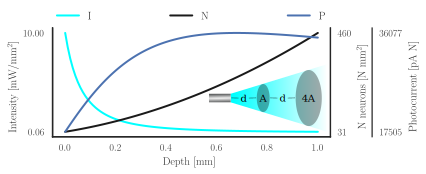
\includegraphics[scale=1]{opto-powerlaw}
\caption{{\bf Spatial extent of optogenetic stimulus}. Due to scattering and geometric loss the light intensity (I, cyan line) plotted as percentage of intensity exiting the optogenetic fiber follows approximately an inverse square law $ r^{-2} $ where $ r $ is the distance from the fiber. If neurons are uniformly distributed the number of affected neurons increase by $ r^{2} $ (N, black line) rendering the probability of activating a neuron approximately constant (IN, blue line). \label{fig:concept}}
\end{figure}

\subsection{Confounding as a problem for the estimation of causal effects}
When we stimulate many neurons at the same time, and observe a post-synaptic neuron to be active after our stimulation, it is hard to know which of the stimulated neurons produced the activity. To illustrate such confounding effects we simulated a network comprised of three neurons (A,B, and C). The neurons receive Poisson spike trains and have added Gaussian white noise to the membrane potential. We also gave them interactions, where spikes of neuron B increase the probability of firing for neuron C but there are no other interactions \cref{fig:intro}\labelcref{fig:intro:1}.
Finally, we allowed simulated optogenetic stimulation to affect neurons A and B (but not C). We thus have a simple system for exploring questions of causality.

After running the simulation, the peri-stimulus time histogram of the stimulated neurons show the result of both the stimulation itself (suppressed for visibility) and the neuron's refractory period \cref{fig:intro}\labelcref{fig:intro:2} (AA, BB).  Since the stimulation affects A and B simultaneously, it induces a strong correlation between A and B \cref{fig:intro}\labelcref{fig:intro:3} (AB). This further generates a strong correlation between A and C, confounding the system by rendering the cross correlation histograms (CCHs) between BC and AC both statistically significant ($ p_{\mathrm{fast}} < 0.001, p_{\mathrm{diff}} < 0.001 $; see \cref{sec:method:cch}) shown in \cref{fig:intro}\labelcref{fig:intro:3}. Even though the correlation peak between B and C is larger than between A and C due to correlated spikes outside the periods with stimulation one may imagine a situation where only A and C is measured, giving rise to a false prediction that they are connected. If stimulation affects multiple neurons simultaneously, there is a real confounding problem.

\begin{figure} 
\makeatletter
\renewcommand\p@subfigure{}
\makeatother
\begin{subfigure}{0.485\textwidth} 
\includegraphics[scale=1]{simple}
\caption{} \label{fig:intro:1}
\end{subfigure}\hfill
\begin{subfigure}{0.485\textwidth} 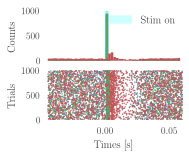
\includegraphics[scale=1]{raster}
\caption{} \label{fig:intro:2}
\end{subfigure}

\medskip
\begin{subfigure}{\textwidth}\centering 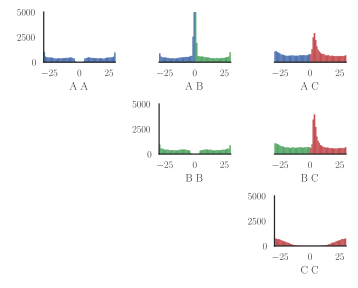
\includegraphics[scale=1]{xcorr}
\caption{} \label{fig:intro:3}
\end{subfigure}
\caption{{\bf A,B,C network}. A sketch of the simple network containing three neurons %depicted in \labelcref{fig:intro:3} 
shows stimulation configuration with blue laser light and the connections with arrows (a). The neurons A and B are stimulated 1000 trials and the corresponding peristimulus time histogram are shown in \labelcref{fig:intro:2} upper panel with a raster plot in the lower panel. Cross correlation histograms (CCHs) are shown in \labelcref{fig:intro:3} where horizontal and vertical axes represents time lag in ms and counts of coincident spikes in bins of 1 ms. \label{fig:intro}}
\end{figure}

\subsection{Instrumental variables to resolve confounding}
In order to estimate the actual influence of stimulation of a neuron on post-synaptic neurons we need something that can distinguish the influence of one stimulated neuron from the influence of another stimulated neuron. We would thus need something that affects the stimulation effect separately between neurons. Arguably, refractoriness is such a variable. If a neuron is in its absolute refractory period, then no amount of stimulation will make it spike. This gives us an interesting way of getting at causality, by comparing the network state between a time when a neuron is able to spike and a time where the neuron is unable to spike.

Instrumental variables requires the existence of a random (or sufficiently random) variable that affects a variable of interest. This independent influence among neurons then allows quantifying the influence of the variable of interest on the rest of the network. In our case, the refractory states of a neuron is in good approximation independent on small time scales (see Discussion for caveats). It affects the influence of stimulation on the potentially pre-synaptic neuron (\cref{fig:cchvswald}\labelcref{fig:cchvswald:0}). The trials where a stimuli is unable to elicit a spike due to the refractory state can then be used to identify causal effect on the potentially post-synaptic neuron.

We can now investigate if the use of an instrumental variable gives a better estimate of connectivity strength than simply analyzing the lagged correlations by means of the CCH; see \cref{eq:ptrans}. We thus use the IV estimator \cref{eq:wald} on the three neuron system (\cref{fig:cchvswald}\labelcref{fig:cchvswald:1,fig:cchvswald:2}). It converges to the correct causal conclusions that the weights $ w_{BC} = 0.2 $ and $ w_{AC} = 0 $. For such a simple system, it produces meaningful estimates of the causal interactions between neurons.

\begin{figure}
\makeatletter
\renewcommand\p@subfigure{}
\makeatother
\begin{subfigure}{0.485\textwidth} \centering
% * <tristan.stoeber@posteo.net> 2018-06-24T21:23:23.987Z:
% What is S?
% ^.
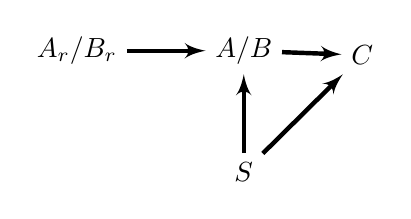
\begin{tikzpicture}
    \node (u) {$ S $};
    \node [above = of u] (x) {$ A/B $};
    \node [above right = of u] (y) {$ C $};
    \node [left = of x] (sr) {$ A_r/B_r $};
    \path [line] (x) -- (y);
    \path [line] (u) -- (x);
    \path [line] (u) -- (y);
    \path [line] (sr) -- (x);
\end{tikzpicture}
\caption{} \label{fig:cchvswald:0}
\end{subfigure}\hfill
\begin{subfigure}{0.485\textwidth} \centering
\includegraphics[scale=1]{wald_legend}
\end{subfigure}\medskip

\begin{subfigure}{0.485\textwidth} 
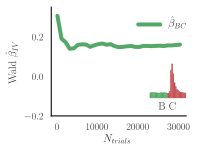
\includegraphics[scale=1]{wald_BC}
\caption{} \label{fig:cchvswald:1}
\end{subfigure}\hfill
\begin{subfigure}{0.485\textwidth} 
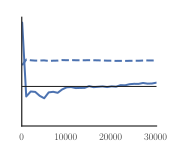
\includegraphics[scale=1]{wald_AC}
\caption{} \label{fig:cchvswald:2}
\end{subfigure}
\caption{{\bf Instrumental variable estimation (IV) of connectivity}. \labelcref{fig:cchvswald:0} In an instrumental variable estimation procedure we use a variable that is assumed to be random (here refractoriness) which influences a variable of interest (here spiking) and to use this influence to infer the causal interaction of that variable on other variables (here spiking of A or B onto C). \labelcref{fig:cchvswald:1} A popular estimation approach for IVs,  the Wald technique correctly estimates causal connectivity in the A,B,C neural network using the refractory period. Subfigure \labelcref{fig:cchvswald:0} shows a path diagram \citep{wright1921correlation} between the upstream neuron $ A $ or $ B $, the stimulation $ S $, the post-synaptic neuron $ C $ and the IV as $ A_{r} $ or $ B_{r} $. Arrows represent associations where $ S $ is associated with $ A,B $ and potentially also with $ C $ both directly and through $ A,B $. The IV estimator calculated by \cref{eq:wald} converges to $ \hat{\beta}_{BC} \approx 0.2, \hat{\beta}_{AC} \approx 0 $ after approximately $ 5000 $ trials as seen in \labelcref{fig:cchvswald:1,fig:cchvswald:2} respectively. % I would have put in a take home message / interpretation of the results in the figure text.
Insets represent high resolution zoom of cross correlation histograms of BC and AC where horizontal and vertical axes represents time lag and counts of coincident spikes in bins of 0.1 ms respectively. \label{fig:cchvswald}}
\end{figure}

\subsection{Larger simulated networks}
The interacting neurons in a biological network exhibit inhibition and interact in many kinds of ways. To evaluate the IV method in a more meaningful setting we thus simulated a recurrent neural network consisting of 1250 randomly connected leaky integrate and fire neurons where 250 had inhibitory synapses. The network was tuned to be in an asynchronous regime; see \cref{fig:state}\labelcref{fig:CC} with log-normally distributed synaptic weights according to patch clamp experiments \citep{Sayer1990,Mason1991}; see \cref{fig:state}\labelcref{fig:syn_dist} and \cref{tab:params} for parameters. Further, we selected 800 excitatory neurons for stimulation and gave each neuron a random spatial distance from the simulated optogenetic stimulus. The stimulus intensity was then set according to \cref{eq:intensity} with a maximum of 10 pA, and was constant throughout trials. The trial onset had a temporal Poisson distribution with period 100 ms and was further clipped between 100-150 ms. For weight estimates we randomly selected among the excitatory population 50 stimulated neurons and 50 unstimulated neurons. 

To evaluate how well the IV method estimates the weights as a function of number of trials we calculated the mean squared error of the weight connecting the 100 neuron pairs \cref{fig:error}. As seen here, the IV estimator's precision decreases similarly in three different settings with varying amounts of relative inhibition $ g $.
\begin{figure}
\makeatletter
\renewcommand\p@subfigure{}
\makeatother
\begin{subfigure}{\textwidth} 
\includegraphics[scale=1]{network-raster}
\caption{} \label{fig:error:raster}
\end{subfigure}\medskip

\begin{subfigure}{\textwidth} 
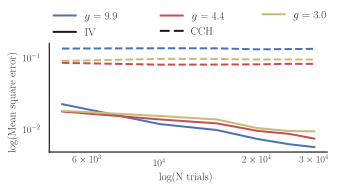
\includegraphics[scale=1]{mse_pos}
\caption{} \label{fig:error:mse}
\end{subfigure}
\caption{{\bf Mean square error (MSE) of IV estimator in a large network}. \labelcref{fig:error:raster} Excitatory neurons (in blue raster) are stimulated with varying intensity indicated by the y-axis in lower panel, upper panel shows inhibitory neurons (red raster) where y-axis indicate random neuron-id. \labelcref{fig:error:mse} The IV- and CCH estimator is evaluated for the asynchronous recurrent neural network at three different amounts of relative inhibition $ g $. The MSE as a function of number of trials is shown on a logarithmic scale where the slopes was found to be $ -0.77, -0.48, -0.40 $ for $g = 9.9, 4.4, 3.0$ respectively. \label{fig:error}}
\end{figure}

We want to compare the IV estimator which exploits the refractory period with the CCH method given by \cref{eq:ptrans} which ignores network confounding. To indicate the amount of connections which are falsely attributed a non-zero weight we calculated the amount of false positives. This was given as the percentage of estimated synapses larger than $ 0.05 $ where the true weight was $ 0 $, finding $ 13.3\% $ for CCH and $ 0.2\% $ for the IV estimator; see \cref{fig:network-class}\labelcref{fig:network-class:1}. In addition we compared the size of the estimations at false positive instances and found that the CCH have slightly higher median. The IV approach, while not being perfect, thus outperforms the simple CCH approach.

It might be that modeling refractory periods in the context of a naive regression estimates connectivity equally well as the IV method. We thus performed a logistic regression as seen in \cref{fig:network-class}\labelcref{fig:network-class:1} denoted LOGIT. As seen here, LOGIT performs even worse than CCH showing that it really helps to use the refractory period as an instrumental variable. To further evaluate the methods we calculated false negatives as instances where the true weight is non-zero but estimated to be equal to zero in \cref{fig:network-class}\labelcref{fig:network-class:2} showing that the CCH and IV estimators performs equally well. Finally we wanted to evaluate the estimated weights as a function of true weights shown in \cref{fig:network-class}\labelcref{fig:network-class:3,fig:network-class:4} after 30000 trials. The IV estimator yields a good prediction $ r^2 = 0.55 $, while the CCH estimator performs surprisingly bad with $ r^2 = 0.002 $. Utilizing refractory periods as an (imperfect) instrumental variable considerably improves estimates.

\begin{figure}
\makeatletter
\renewcommand\p@subfigure{}
\makeatother
\begin{subfigure}{0.485\textwidth} 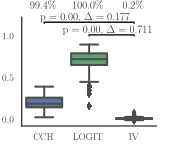
\includegraphics[scale=1]{false_positive}
\caption{} \label{fig:network-class:1}
\end{subfigure}\hfill
\begin{subfigure}{0.485\textwidth} 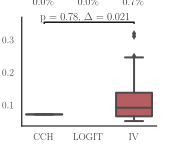
\includegraphics[scale=1]{false_negative}
\caption{} \label{fig:network-class:2}
\end{subfigure}
% * <tristan.stoeber@posteo.net> 2018-06-24T21:29:41.690Z:
% 
% Why is logit not considered for false negatives?
% 
% ^.

\medskip
\begin{subfigure}{0.46\textwidth} 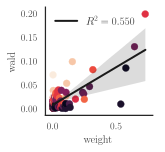
\includegraphics[scale=1]{fit_wald_pos}
\caption{} \label{fig:network-class:3}
\end{subfigure}\hfill
\begin{subfigure}{0.6\textwidth} 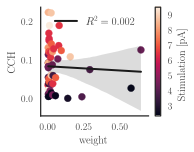
\includegraphics[scale=1]{fit_cch_pos}
\caption{} \label{fig:network-class:4}
\end{subfigure}
\caption{{\bf False estimates and goodness of fit}. False positives are shown in \labelcref{fig:network-class:1} for the cross correlation histogram (CCH) method, logistic regression (LOGIT) and the IV estimator. False negatives for CCH and IV is shown in \labelcref{fig:network-class:2}. Positive estimates of weight as a function of true weight is scattered for the IV estimator in \labelcref{fig:network-class:3} and CCH in \labelcref{fig:network-class:4} color coded by the size of perturbation intensity. Shaded area show the 95 \% confidence interval calculated by bootstrapping.
\label{fig:network-class}}
\end{figure}

\section{Discussion}
%% maybe add somewhere that using other recorded neurons may be useful as well.

Here we have asked if the refractory period of neurons can be used as an instrumental variable to reverse engineer the causal flow of activity in a network of simulated neurons. We have found that this approach performs considerably better than the naive method. We have found that neither naive linear nor naive logit models produce good estimates of weights. Our system effectively reverse engineers causality by looking at the response that is missing because of refractoriness which effectively allows better estimates of causal effects. 

%Wald is pairwise, GLMs require multiple neurons
One popular way of estimating causal effects is fitting generalized linear models (GLMs) to simultaneously recorded neurons \citep{pillow2008spatio}. The GLMs are basically multiple regressions and require multiple neurons in order to perform well. In fact, if one recorded all neurons, GLMs could be sufficient to estimate causal connections. However, this is not the case for research in the mammalian brain, especially not for primates, where we only record a very small subset of the neurons that do the actual computation. The GLM field is very strong at modeling latency distributions and sequences of spikes in individual neurons. These ideas should, arguably, be merged with IV approaches. The main strength of the  IV estimator presented here compared with GLM methods is that we only require one pair because we can utilize the randomness in refractoriness. 

%We recommend the WALD, easily usable in the context of many experiment. Potentials for future improvement.
%The IV estimator seems to be useful when using the refractory period. This method yields a direct estimation by computing the difference in mean activity of a putative post-synaptic neuron when the upstream neuron is responsive to the stimulus or not. Moreover, as this method only requires one pair it is easily usable in many types of experiments, with large or small recording counts. However, there would be many ways of improving the estimates, we could better model the temporal sequence of spikes, we could utilize latency in a more meaningful way. While there are many ways of improving the IV estimators, we have here represented the most basic implementation using the Wald estimator.


% Maybe nonlinearities in stimulation rescue old school approaches
% Discuss distribution of V. Discuss 2p stimulation.  Conclude that there is absolutely no reason to hope things will work with 1p.
The main problem with optogenetics when using it to infer connectivity is its non-local property. This is due to the inverse relation between changes in light intensity and affected number of neurons combined with the observation that distribution of membrane potentials across neurons is flat \citep{destexhe1999impact,rudolph2006use,pare1998impact}. One could however imagine situations where optogenetic activation were more local. If membrane potential distributions were in general skewed with the mode far from threshold the optogenetic perturbation would be more local. This is because each neuron would require a very strong stimulus in order to  elicit spikes at all. But there could be other ways of making optogenetics more local. For example, if one could engineer opsins with far more absorbent wavelengths one could stimulate locally. How to engineer more localized stimulation is an important problem if one wants to causally interrogate systems.

%Maybe weak stimulation will rescue us. No way, but cite Buszaki.
Very weak laser pulses in noisy networks might only affect very few neurons each trial \citep{English2017}. However, the stimulus will still affect the many far away neurons by a tiny bit. Therefore, weak stimulation does not remove the principal problem of the CCH estimator. Moreover, the network still acts as a confounder and, if anything, the weak stimulation will dramatically reduce the statistical power of the approach. Lowering stimulation amplitudes does not appear to be a way of obtaining meaningful causal estimates.

%Correlated refractory periods is *the* failure mode. How to randomize them
For the refractory period to be a good instrument, it is necessary that it is not overly affected by the network activity. This clearly is going to be problematic in many cases, after all the network activity affects refractoriness. However, there are multiple scenarios where refractoriness will be a good instrument. For example, if we have balanced excitation and inhibition we may expect largely independent refractory states of individual neurons. If a neuron biophysically implements something like conditional Poisson spiking its refractory states will be random. Even if neurons refractory states are strongly correlated during normal network operation there may be ways of randomizing them. Giving one burst of stimulation which is strong enough to elicit multiple spikes from each neuron may effectively randomize the phase of each neuron \citep{ermentrout2008reliability}. Importantly, we may expect the phase of a neuron to be far more random than the activity of the network as a whole.

%Still some troubles
We found some negative values of the IV estimator which were suppressed as we knew that we only stimulated excitatory neurons. This happens because some neurons  have correlated refractory times which we hypothesize to be mainly due to synchrony induced by the stimulation \citep{ermentrout2008reliability}. This hypothesis was strengthened by observing that this negative values did not occur when the stimulation intensity was set to zero (data not shown). Furthermore, respective simulated neural network introduces much response overlap due to synapses having identical synaptic time constants and transfer delays. This makes inference quite hard since multiple neurons are affecting the same cell at the same time for each stimulation.  However, this is less likely to occur in biological networks, which have high variability of synaptic properties and where firing patterns are sparser. These biological aspects would most likely work to the advantage of the IV method. Independence of refractoriness would be further improved, if in addition a clever stimulation routine was implemented such that the distribution of stimulation strength varies spatially from trial to trial.

% Importance of randomized stimulus times and short pulses 
The independence of refractory times is the one factor which makes or breaks the IV approach. Therefore we may think of ways of making the refractoriness distribution more random. First, it would help to use a task and situation where neurons are as uncorrelated as possible. Second, we may use a set of conditioning pulses of stimulation to increase independence of refractory states. Third, we may utilize chemical, behavioral, or molecular perturbations to randomize refractoriness. There has not, to the authors knowledge, been any attempts in neuroscience to randomize times of refractory states, so there may be a lot of possibilities to improve.

Generalizing this idea, we may ask if there are ways of constructing good instrumental variables. One may assume a way of building molecular oscillators or otherwise pattern generators into neurons which affect their firing rate. Such modulatory activity would be observable in the extracellular activity of the neuron. Any neuron that then correlates to this modulation must be post-synaptic of the recorded neuron. Any kind of a signal that is local to a cell and not affected by network activity could produce a meaningful instrumental variable and it might be reasonably doable to link membrane channels to intracellular signal generation. Even if perfect IVs do not exist in brains, we may be able to make them.

%Causal inference techniques to fix experimental issues
There are many techniques for causal inference and most of them are largely unknown in neuroscience and are based on approximating randomness in a world that does not have it. In many cases, one could use regression discontinuity designs in a spiking system \citep{BenPaper, imbens2008regression}. Moreover, one could use a difference in difference approach \citep{abadie2005semiparametric}. Matching approaches \citep{stuart2010matching}, but see \citep{king2016propensity}, can be used where one compares similar network states and their evolution over time. In general, neuroscience is in a quest for causal interpretations, we should therefore be able to benefit considerably by utilizing techniques that are popular in the field of causal inference.

%Constructing good IVs; Multiple illuminations, designed sticky opsins
% Many trials needed here, good IV could possibly decrease this number
%We note that we obtained low errors from the IV estimator after relatively few trials when estimating weights in the neural network of 1250 neurons.\todo{how would this be in the brain with more variable synaptic properties?} This amount of trials is not experimentally possible and we therefore foresee the need for improvements of the IV method. It can be improved in two ways, either with algorithms that uses more of the information available, such as the exact stimulus latencies and/or the amount of spikes in each trial. The other improvement could be to design experimental procedures that open for causal interpretation. 

%If we assume that the assumption of random refractory periods are violated somehow by the physiology, e.g.a very synchronized network. To ameliorate one could introduce multiple light sources that is activated in a randomized fashion such that the intensity distribution is randomized. This could be realized with e.g. laser holograms/filter or multiple micro LEDs This would in addition increase the amount of neurons targeted and thus give larger experimental yield. Another possibility is to design opsins that have a fluctuating baseline levels randomizing membrane potential of affected neurons, however this could also lead to a chronic deficit in respective neural network and would thus shorten the time span of the experimental procedure. But importantly, designing experiments so that causal inference is possible should be a major consideration for experimental design.

\section{Methods}
\subsection{Instrumental variable estimation}
A simple approximation of the connectivity strength between a pre-synaptic neuron $ x $ and post-synaptic neuron $ y $ can be to ignore external excitation and simply calculate the relation between the spike times in $ x $ and $ y $ with a regression model given by

\begin{equation}
y = \beta x + u.
\label{eq:regress}
\end{equation}
Here $ y $ is the dependent variable, $ x $ is the explanatory variable, $ \beta $ is the effect of the $ x$ on $y $ and $ u $ is an unknown error term. \Cref{eq:regress} follows from the causal path diagram (invented by \cite{wright1921correlation})
\begin{center}
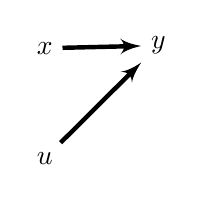
\begin{tikzpicture}
    \node (u) {$ u $};
    \node [above = of u] (x) {$ x $};
    \node [above right = of u] (y) {$ y $};
    \path [line] (x) -- (y);
    \path [line] (u) -- (y);
\end{tikzpicture}
\end{center}
Assuming that changes in spike times $ y $ are described by $ \beta x $ i.e. $ \de{y}{x} = \beta $ for spike times $ x $. One problem with this idea is that in a confounded system, perfectly correlated neurons will give statistically indistinguishable $ \beta $. In the extreme case where two neurons are both made to fire every time they are stimulated, they will have the same weights according to \cref{eq:regress}. After all, during stimulation $ y=1 $ for both, even if only one of them drives the post-synaptic neuron. Another problem is if the network state affects both the probability of a neuron to fire and also the probability of post-synaptic neurons to fire. In this case, the network state can induce a correlation which will make the estimation highly biased. Arguably, the network state will, in all realistic models, have a dramatic influence on all neurons and the regression model is better described by
\begin{equation}
y = \beta x + u(x).
\end{equation}
Corresponding to the following path diagram

\begin{center}
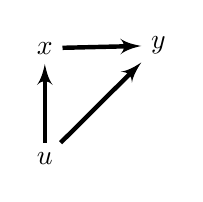
\begin{tikzpicture}
    \node (u) {$ u $};
    \node [above = of u] (x) {$ x $};
    \node [above right = of u] (y) {$ y $};
    \path [line] (x) -- (y);
    \path [line] (u) -- (x);
    \path [line] (u) -- (y);
\end{tikzpicture}
\end{center}
Here we have the relation $ \de{y}{x} = \beta + \de{u}{x} $. To get at causality we thus require some stimulation that only highlight the activity in $ y $ caused by $ x $, disassociating $x$ from $u$. However, the optogenetic stimulation is not specific to $x$ and will activate parts of the network activity $ u $. Let us assume that the stimulus renders only a subset of $u$ correlated with $x$, namely $u_s$ ($s$ denotes stimulated). To disassociate $x$ from $u_s$ we need something that can distinguish between different neurons that are stimulated. We thus require some instrument $ x_{s_r} $ which is (1) uncorrelated with the network $ u $ and (2) is correlated with the regressor $ x $ \citep{angrist2008mostly}. We assume that the neurons are independent at small time scales and that stimulation additionally randomize membrane potential individually in neurons. We may thus use the fact that a neuron that has fired just before the stimulation will be in an absolute refractory state and hence have $ x_{s_r}=0 $ independently of $u$, where the subscript $s_r$ denotes stimulation during refractory state. This introduces times where the spike from one of the stimulated neurons are missing. Thus we may use the refractory period as an instrumental variable, as illustrated with the following path diagram

\begin{center}
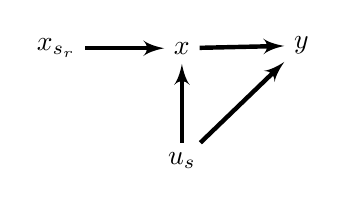
\begin{tikzpicture}
    \node (u) {$ u_s $};
    \node [above = of u] (x) {$ x $};
    \node [above right = of u] (y) {$ y $};
    \node [left = of x] (sr) {$ x_{s_r} $};
    \path [line] (x) -- (y);
    \path [line] (u) -- (x);
    \path [line] (u) -- (y);
    \path [line] (sr) -- (x);
\end{tikzpicture}
\end{center}
Here $ x_r $ represent times where the pre-synaptic neuron is refractory during stimulation. This is then an estimator that compares the post-synaptic activity when a given neuron is non-refractory with the post-synaptic activity when it is refractory, thus removing the confounding. The true $ \beta $ is given by
% * <tristan.stoeber@posteo.net> 2018-06-24T22:11:38.685Z:
% Shouldnt it be  $ x_s_r $
% ^.
\begin{equation}
\beta_{IV} = \de{y}{x_{s_r}} / \de{x}{x_{s_r}}
\end{equation}
Since our instrument $ x_{s_r} $ is binary we may use the IV (or more precisely Wald) estimator \citep{wald1940fitting} to estimate $ \beta_{IV} $ by
\begin{equation}
 \hat{\beta}_{IV} = \frac{\bar{y}_{s} - \bar{y}_{s_r}}{\bar{x}_{s} - \bar{x}_{s_r}} = \bar{y}_{s} - \bar{y}_{s_r}
 \label{eq:wald}
\end{equation}
Here $ \bar{y}_s $ is the average number of trials where successfully stimulating $ x $ resulted in a response in $ y $ and $ \bar{y}_{s_r} $ is the average number of trials where an unsuccessful stimulation of $x$ resulted in a response in $ y $. The successful stimulations of $x$ are denoted $x_s$ and thus  $\bar{x}_s \equiv 1$. Conversely $x_{s_r}$ denotes unsuccessful stimulations of $x$ i.e. stimulations of $x$ during its refractory state and $\bar{x}_{s_r} \equiv 0$.

To utilize the refractory period as an IV we first picked out one window of $ 4 $ ms for each of the pre-synaptic and post-synaptic neuron with a latency relative to stimulation time of $ 0 $ and $ \tau_{syn} + D $ ms (see \cref{eq:syn}) respectively. By classifying each window for each trial whether $x$ contained a spike we obtained the two binary arrays $ y_s $ and $ y_{sr} $.

\subsection{Cross correlation histogram}\label{sec:method:cch}
The statistical tests giving the probabilities $ p_{diff} $ and $ p_{fast} $ were done according to \cite{Stark2009, English2017}. Briefly, to test if the cross correlation histogram (CCH) peak was significant we employed two tests. By using the Poisson distribution with a continuity correction \citep{Stark2009} given by \cref{eq:poissoncontcor} we calculated $ p_{diff} $ by comparing the peak in positive time lag with the maximum peak in negative time lag \citep{English2017}. The probability $ p_{fast} $ represents the difference between CCH and it's convolution with a hollow Gaussian kernel \citep{Stark2009}.
\begin{equation}
p(N|\lambda(m)) = 1 - \sum_{k=0}^{N-1}\frac{e^{-\lambda(m)}\lambda(m)^k}{k!} - \frac{e^{-\lambda(m)}\lambda(m)^N}{2N!}
\label{eq:poissoncontcor}
\end{equation}
Here $ \lambda $ represents the counts at bin $ m $ and $ N $ is the number of bins considered. To estimate the connection weight between pairs we used the spike transmission probability defined in \cite{English2017} as 
\begin{align}
\label{eq:ptrans}
P_{trans} = \frac{1}{n}\sum_{m=3ms}^{6ms} CCH(m) - \lambda_{Gauss}(m),
\end{align}
where $ n $ is the number of spikes detected in the presynaptic neuron and $\lambda_{Gauss}(m)$ is the CCH count convolved with a hollow Gaussian kernel at bin $m$.

\subsection{Logistic regression}
To utilize the refractory period without using it as an IV we estimated synaptic weights using a logistic regression. To do this we first picked out one window of $ 4 $ ms for each of the pre-synaptic and post-synaptic neuron with a latency relative to stimulation time of $ 0 $ and $ \tau_{syn} + D $ ms (see \cref{eq:syn} ) respectively. By classifying each window for each trial whether it contained a spike we obtained two binary arrays, the regressor $ x $ and the dependent variable $ y $ where we want to estimate the probability $ P(y = 1|x) $ by fitting the parameters $ \vec{\beta} $ such that
\begin{align}
y = \begin{cases}
	1 & \text{if } \beta_0 + \beta_1x + u > 0\\
    0 & \text{else}
\end{cases}
\end{align}
where $ u $ is an error term. Further, we used the logit link function such that the the probability giving the proxy for synaptic weight is given by
\begin{align}
p(x) = \frac{1}{1 + e^{-(\beta_0 + \beta_1x)}}
\end{align}
The model was fitted using the python package scikit-learn \citep{scikit-learn}

\subsection{Simulated network}
To simulate a recurrent network of excitatory and inhibitory neurons we used the leaky integrate and fire (LIF) model given by
\begin{equation}
	\de{V_m^i}{t} = - \frac{(V_m^i - E_L)}{\tau_m} + \frac{I_{syn}^i(t)}{C_m}.
    \label{eq:LIF}
\end{equation}
When the membrane potential $ V_m^{i} $ of neuron $ i $ reaches a threshold $ V_{th} $ an action potential is emitted and $ V_m^{i} $ reset to the leak potential $ E_{L} $ followed by an absolute refractory period $ \tau_{ref} $. The membrane time constant is represented by $ \tau_{m} $ and $ I_{syn}^{i}(t) $ denotes the post synaptic current (PSC) for neuron $ i $ modeled as a sum of alpha functions given by
\begin{equation}
	\label{eq:syn}
	I_{syn}^i(t) = \sum_{j=1}^C J_j \alpha(t - t_j - D),
\end{equation}
where $ t_j $ denotes an incoming spike through synapse $ j $ at delay $ D $ and $ C $ is the number of incoming synapses on neuron $ i $. The PSC amplitude is given by $ J_{j} $ and the alpha function is given by
\begin{align}
\tau_{syn}\alpha(t) = te^{-\frac{t}{\tau_{syn}}} H(t).
\end{align}
Here $ \tau_{syn} $ denotes the synaptic integration time constant and $ H $ is the Heaviside step function. All neurons were driven by an external Poisson process with rate $ rate_{p} $.

Synaptic weights were log-normally distributed such that the increase in membrane potential $ V_m^i $ due to one spike were restricted to lie between $ V_{syn} = 0.05 mV $ and $ V_{syn} = 2.05 mV $ based on experimental findings \citep{Sayer1990,Mason1991}. The synaptic distribution is shown in \cref{fig:state}\labelcref{fig:syn_dist} where the inhibitory PSC amplitude is given by $ J_{in} = g J_{ex} $ where $ J_{ex} $ denotes the excitatory synaptic weight.

To find suitable parameters yielding asynchronous activity we measured the population correlation coefficient given by

\begin{align}
\mean{CC}_{pop} = \mean{\mean{\frac{h_{i} - \mean{h_{i}}}{std(h_{i})}\frac{h_{j} - \mean{h_{j}}}{std(h_{j})}}}_{pop},
\end{align}
where $ h $ is the spike time histogram with binsize at $ 5ms $ for neuron $ i,j $ and $ \mean{\cdot} $ is the mean operator. The distribution of $ CC $ is shown in \cref{fig:cchvswald} which were found by performing several parameter sweeps picking three parameter sets which mainly differed in firing rate (data not shown). 

To further evaluate the network state we calculated the coefficient of variation (CV) of the population given by
\begin{align}
\mean{CV} = \mean{\frac{std(ISI_i)}{\mean{ISI_i}}}_{pop},
\end{align}
where $ ISI $ denotes the inter-spike interval of neuron $ i $. Due to the finite time synaptic integration time constant $ \tau_{syn} = 1 ms $ we were unable to have the network showing an irregular state; see \cref{fig:state}\labelcref{fig:CV}. To verify that indeed this was due to $ \tau_{syn} $ we performed several simulations with lower $ \tau_{syn} $ obtaining $ \mean{CV}_{pop} > 1 $ (data not shown). It would likely be easier to achieve irregular network state if synapses were conductance based \citep{Kumar2008}. However, we settled with current based synapses as we were mainly interested in achieving an asynchronized state ($ \mean{CC}_{pop} < 0.01 $).
\begin{figure}
\makeatletter
\renewcommand\p@subfigure{}
\makeatother
\begin{subfigure}{0.485\textwidth} 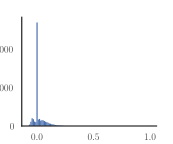
\includegraphics[scale=1]{CC}
\caption{} \label{fig:CC}
\end{subfigure}\hfill
\begin{subfigure}{0.485\textwidth} \includegraphics[scale=1]{CV}
\caption{} \label{fig:CV}
\end{subfigure}\medskip

\begin{subfigure}{\textwidth}\centering 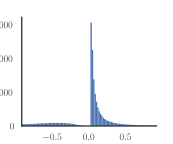
\includegraphics[scale=1]{syn_dist}
\caption{} \label{fig:syn_dist}
\end{subfigure}
\caption{Network state \label{fig:state}}
\end{figure}

\begin{table}
\begin{tabular}{lllll}
\toprule
{} &    model 1 &    model 2 &    model 3 &       units \\
\midrule
$N_{neurons}$         &       1250 &        &        &             \\
$\Delta t$            &        0.1 &         &         &             \\
$N_{ex}$              &       1000 &        &        &             \\
$N_{in}$              &        250 &         &         &             \\
$eta$                 &        0.9 &         &         &             \\
$rate_{p}$            &    3694.26 &          &     &          Hz \\
$V_{reset}$           &          0 &           &           &          mV \\
$V_{m}$               &          0 &           &           &          mV \\
$E_{L}$               &          0 &           &           &          mV \\
$t_{ref}$             &          2 &           &           &          ms \\
$\tau_{m}$            &         20 &          &          &          ms \\
$V_{th}$              &         20 &          &          &          mV \\
$C_{m}$               &          1 &           &           &          pF \\
$V_{syn}$             &        0.2 &         &        &          mV \\
$g$                   &        9.9 &        4.4 &          3 &             \\
$V_{syn}^{high}$      &       2.05 &        &        &          mV \\
$V_{syn}^{low}$       &       0.05 &        &       &          mV \\
$var_{syn}$           &        0.5 &         &         &      mV$^2$ \\
$\tau_{syn}^{in}$     &          1 &           &           &          ms \\
$\tau_{syn}^{ex}$     &          1 &           &           &          ms \\
$delay$               &        1.5 &         &        &          ms \\
$eps$                 &        0.1 &        &         &             \\
$C_{ex}$              &        100 &         &         &             \\
$C_{in}$              &         25 &          &          &             \\
$J_{in}$              &    0.88727 &   0.394342 &    0.26887 &          pA \\
$J_{ex}$              &  0.0896232 &   &   &          pA \\
$J_{high}^{ex}$       &   0.918638 &    &    &          pA \\
$J_{low}^{ex}$        &  0.0224058 &   &   &          pA \\
$J_{high}^{in}$       &   0.918638 &    &   &          pA \\
$J_{low}^{in}$        &  0.0224058 &   &   &          pA \\
$stim_{N}^{in}$       &          0 &           &           &             \\
$stim_{N}^{ex}$       &        800 &         &         &             \\
$stim_{amp}^{in}$     &          0 &           &           &          pA \\
$stim_{amp}^{ex}$     &         10 &          &          &          pA \\
$stim_{duration}$     &          2 &           &           &          ms \\
$stim_{period}$       &        100 &         &         &          ms \\
$stim_{max}^{period}$ &        150 &         &         &          ms \\
$rate_{in}$           &    7.17024 &    9.66335 &     11.754 &          Hz \\
$rate_{ex}$           &    9.05793 &    10.9176 &    13.1032 &          Hz \\
$density$             &     100000 &      &      &  Nmm$^{-3}$ \\
$S$                   &       10.3 &       &      &   mm$^{-1}$ \\
$NA$                  &       0.37 &       &       &             \\
$r$                   &        0.1 &         &         &      $\mu$m \\
$n$                   &       1.36 &        &        &             \\
\bottomrule
\end{tabular}
\caption{\label{tab:params} Simulation parameters of three different models.}
\end{table}

\subsection{Perturbation intensity}\label{sec:method:opto}
In order to replicate an optogenetic experiment we modeled transmission of light through brain tissue with the Kubelka-Munk model for diffuse scattering in planar, homogeneous, ideal diffusing media given by
\begin{align}
T = \frac{1}{Sz + 1}.
\end{align}
Here $ T $ denotes a transmisison fraction, $ S $ is the scattering coefficient for mice \citep{Aravanis2007} and $ z $ is the distance from a light source \citep{Ho2017}. Further we combined diffusion with geometric loss assuming that absorption is negligible as in \cite{Aravanis2007} and computed the intensity as presented in \cref{fig:concept} by
\begin{align}
\label{eq:intensity}
\frac{I(r)}{I(r=0)} = \frac{\rho^2}{(Sr + 1)(r + \rho)^2}
\end{align}
where $ r $ is the distance from the optical fiber and
\begin{align}
\rho = \frac{d}{2}\sqrt{\left(\frac{n}{NA}\right)^2 - 1}.
\end{align}
Here $ d $ is the diameter of the optical fiber, $ NA $ is the numerical aperture of the optical fiber and $ n $ is the refraction index for gray matter \citep{Ho2017}; see numerical values for parameters in \cref{tab:params}.

To estimate the distribution of light intensity on affected neurons we assumed a neuron density of $ 10^4 Nmm^{-3} $ and found the volume of a cut cone that could contain the number of stimulated excitatory neurons which were found to yield the depth $ r_{max} = 0.175 mm $. We then selected $ N_stim $ neurons that were given a random position in the range $ [0, r_{max}] $ and were assigned a stimulation strength as the maximum stimulation strength multiplied by \cref{eq:intensity}. Then we selected $ 50 $ of the excitatory neurons that were not stimulated as the ``target" population which together with the inhibitory neurons were not perturbed directly by the light stimulus.

In order to keep the stimulus model as simple as possible we let set the maximum stimulation strength to $ 10 pA $ which was found suitable by investigating the percentage of successful stimulations to be around $ 50\% $.

%-------------------------------------------------------------------------------
%                                 REFS
%-------------------------------------------------------------------------------
\pagestyle{empty}
\bibliographystyle{apalike}
{\footnotesize\linespread{1}
\bibliography{library}}
%-------------------------------------------------------------------------------
%                                 TODOS
%-------------------------------------------------------------------------------
%\newpage
%\listoftodos
\end{document}
